\chapter{Implementación ...}
\label{Implementacion}

...

\section{Análisis de los Lenguajes de Transformación de Modelos}\label{Analisis de los Lenguajes de Transformacion de Modelos}

En esta sección se analizan las propuestas existentes con el fin de fundamentar la elección del lenguaje utilizado en el actual trabajo.
El cuadro \ref{tabla:lenguajesdetransformacion} es una muestra de sólo algunos de una diversidad de lenguajes de transformación que se pueden
encontrar en la actualidad. Se muestra el gran número de propuestas existentes, que evidencia el gran interés que se ha despertado por este aspecto
del paradigma del desarrollo de software dirigido por modelos, así como la enorme actividad de investigación surgida alrededor del mismo.\\

\begin{table}[!hbt]
\begin{center}
\footnotesize
\begin{tabular}{| p{4cm}| p{8cm}|}
\hline
\textbf{Lenguaje/Implementación} & \textbf{Breve Descripción}\\
\hline
ATL (Atlas Transformation Language)  & Lenguaje de transformación de modelos y herramienta para Eclipse desarrollada por el Atlas Group (INRIA).\\
\hline
BOTL(Basic Object-Oriented Transformation Language) & Propuesta gráfica de la Universidad Técnica de München.\\
\hline
ETL (Epsilon Transformacion Language) &  Lenguaje definido sobre la plataforma Epsilon, plataforma desarrollada como un conjunto de plug-ins (editores, asistentes, pantallas de configuración, etc.) sobre Eclipse. Dicha plataforma presenta el lenguaje de metamodelado independiente Epsilon Object Language que se basa en OCL, y puede ser utilizado como lenguaje de gestión de modelos o como infraestructura a extender para producir nuevos lenguajes específicos de dominio, como el citado Epsilon Transformation Language (ETL). Además de ETL, Epsilon soporta a Epsilon Compari\-son Language (ECL) y a Epsilon Merging Language (EML), orientados a la comparación y composición de modelos, res\-pectivamente.\\
\hline
M2T (Model to Text project)  & Se focaliza en la generación de artefactos textuales a partir de modelos. Consta de un conjunto de herramientas desarrolladas para la plataforma Eclipse.\\
\hline
MTF (Model Transformation Framework) & Es un conjunto de herramientas desarrollado por IBM que permiten hacer comparaciones, comprobar la consistencia y ejecutar transformaciones entre modelos EMF.\\
\hline
MTL (Model Transformation Language) & Lenguaje de transformación de modelos y herramienta en Eclipse desarrollada por el grupo Triskell.\\
\hline 
QVT (Query/View/Transformation) & Especificación estándar de OMG. Está basado en MOF (Meta Object Facility) para lenguajes de transformación en MDA. 
Implementaciones: 
\begin{tabular}{p{2,5cm} p{4.7cm}}
QVT$-$Operational: & QVT Operacional de Borland\\
 & SmartQVT \\
 & Eclipse M2M\\
QVT-Core: & OptimalJ (Descontinuado)\\
 & QVT-Relations: \\
 & \hspace{0.5cm} MediniQVT\\
 & \hspace{0.5cm} Eclipse M2M Declarative QVT\\
 & \hspace{0.5cm} ModelMorf\\
\end{tabular}

\\  
\hline
 RubyTL & Lenguaje de transformación híbrido definido como un lenguaje específico del dominio embebido en el lenguaje de programación Ruby. Diseñado como un lenguaje extensible en el que un mecanismo de plugins permite añadir nuevas características al núcleo de características básicas.\\   

\hline
\end{tabular}
\caption{Lenguajes de transformación de modelos.}
\label{tabla:lenguajesdetransformacion}
\end{center}
\end{table}
\normalsize

Existe una variedad muy amplia de lenguajes de transformación, donde cada uno posee características deseables al igual que inconvenientes. Los lenguajes específicos del dominio (Domain Specific Language - DSL), como MT, ofrecen la ventaja de aprovechar todo el potencial del lenguaje \emph{host}, sumándole la expresividad y sofisticación del aparato transformacional. No obstante, esta característica también los hace poco compatible con otras herramientas que se basen en los estándares de la OMG (QVT, OCL, MOF, etc). Por otra parte, los lenguajes gráficos como UMLX son sumamente intuitivos pero a la vez limitados por la misma conformación de la simbología del lenguaje. Conjuntamente, la descripción de una transformación demasiada compleja puede resultar engorrosa para su utilización. Además, suelen incurrir en costos computacionales más elevados en comparación con lenguajes textuales, debido especialmente a que su representación es más compleja de procesar por su naturaleza gráfica. Los lenguajes de 
transformación M2T son bastante útiles para realizar implementaciones específicas de plataforma a partir de un modelo independiente de plataforma. Sin embargo, dejan de lado la transformación entre modelos, parte fundamental del desarrollo de software dirigido por modelos. En cualquier caso, actualmente muchas de las propuestas analizadas se encuentran en etapa de desarrollo, lo cual seguramente permitirá observar, en el futuro, mejoras en cada una de ellas.\\

QVT y los basados en éste, como por ejemplo ATL, tienen la ventaja de ceñirse a un estándar, lo cual los hace mas compatibles con otras tecnologías y comprensibles dada la formalidad de su especificación. Además, múltiples herramientas se han desarro\-llado que dan soporte a su implementación, entre ellas MEDINIQVT, la cual es una de las más robustas en la actualidad. Bajo las consideraciones mencionadas y otras comparativas efectuadas el lenguaje seleccionado para el actual trabajo es QVT.


\section{Lenguaje Query/View/Transformation Relations}
\label{Lenguaje Query/View/Transformation (QVT)}

La OMG ha definido el estándar Query/View/Transformation (QVT) \cite{QVT10} para utilizar en los procesos de desarrollo de software guiados por modelos. QVT consta de tres partes: consulta, vista y transformaciones. El componente de consultas de QVT toma como entrada un modelo y selecciona elementos específicos del mismo. Para la reso\-lución de las consultas y res\-tric\-ciones sobre los modelos, se propone el uso de una versión extendida de OCL 2.0 \cite{OCL20}. La parte de vista es una proyección realizada sobre un modelo y es creada mediante una transformación. Una vista puede verse como el resultado de una consulta sobre un modelo, ofreciendo como resultado un punto de vista de éste, restringiéndolo de acuerdo a alguna condición impuesta. 
En esta sección se presenta el componente de transformaciones de QVT que tiene como objetivo definir transformaciones. Estas transformaciones describen relaciones entre un metamodelo fuente \emph{F} y un metamodelo objetivo \emph{O}. Ambos metamodelos deben estar especificados con el estándar Meta-Object Facility (MOF) \cite{MOF11}. Una vez definida la transformación en QVT, ésta puede ejecutarse para obtener un modelo objetivo, que es una instancia del metamodelo \emph{O} a partir de un modelo fuente, el cual es una instancia del metamodelo \emph{F}.\\

La especificación de QVT 1.0 \cite{QVT10} tiene una naturaleza híbrida declarativa/im\-perativa, donde la parte declarativa se divide en una arquitectura de dos niveles
(ver figura \ref{fig:qvt}) constituida por un metamodelo y un lenguaje llamado \emph{Relations} que sigue un paradigma declarativo, el cual soporta 
concordancia de patrones (Pattern Matching) de objetos complejos y plantillas de creación de objetos, y un metamodelo y un lenguaje llamado \emph{Core}, 
definido usando mínimas extensiones de MOF y OCL.  En este trabajo se hace uso del lenguaje \emph{Relations} que permite especificar relaciones entre 
metamodelos MOF y de la herramienta para la definición de las transformaciones MediniQVT \cite{MED11}. 
Esta herra\-mienta implementa la especificación QVT/Relations en un poderoso motor QVT. Está diseñada para transformaciones de modelos permitiendo un 
rápido desarrollo, mantenimiento y particulari\-zación de reglas de transformación de procesos específicos. Su interfaz está basada en Eclipse y 
utiliza Eclipse Modeling Framework (EMF) \cite{EMF10} para la representación de los modelos. Además, posee un editor con asistente de código y un 
depurador de relaciones. MediniQVT exige que los metamodelos (y modelos) sean escritos en una variante simplificada del estándar MOF, llamada 
Ecore \cite{ECORE12}, el cual ha sido definido en el EMF.

\begin{figure}[!h] 
\begin{center}
 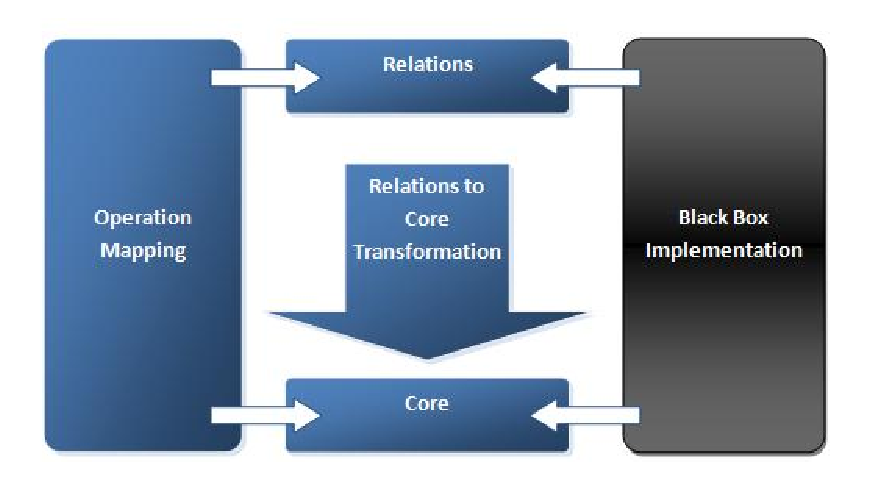
\includegraphics [scale=0.75]{imagenes/qvt.eps}
\end{center}
\caption{Arquitectura QVT.}
\label{fig:qvt}
\end{figure} 

\subsection*{Características de Eclipse Modeling Framework y Ecore}
\addcontentsline{toc}{subsection}{Características de Eclipse Modeling Framework y Ecore} % si queremos que aparezca en el índice

El lenguaje Ecore es el utilizado por el Eclipse Modeling Framework (EMF). Los metamodelos y modelos usados por EMF se representan con documentos XML. Existen herramientas que tratan automáticamente estos metamodelos y modelos. Por ejemplo, EMF ge\-ne\-ra código automáticamente para editores de modelos para un lenguaje de mode\-lado, definido con un metamodelo en Ecore. Otro ejemplo es el plug-in de Eclipse para transformar este tipo de modelos, con la definición de transformaciones QVT. Los metamodelos de Ecore son XML, sin embargo EMF posee un editor gráfico de modelos Ecore que facilita su creación.\\

Las características y elementos del lenguaje de modelado Ecore son los sigui\-entes: el elemento aglutinador (raíz) es el paquete \texttt{EPackage}, que contiene físicamente a sus elementos (especificación de
\texttt{containment}) y, a su vez, éstos pueden estar contenidos en otros paquetes. Hay una fábrica (\texttt{EFactory}) por paquete que permite la creación de los elementos del modelo. Las construcciones que describen a un conjunto de elementos (instancias) son clasificadores (\texttt{EClassifiers}): \texttt{EClass} y \texttt{EDataType}.\\

Ecore especifica las características de las clases (\texttt{EClass}), sus características estructurales (\texttt{EStructuralFeatures}), atributos (\texttt{EAttributes}), operaciones y relaciones (herencia, referencia (\texttt{EReference})). Las \texttt{EClasses} tienen superclases y están compuestas por características estructurales (\texttt{EStructuralFeatures}: \texttt{EReference} y \texttt{EAttribu\-te}). Tanto las \texttt{EReferences} como los \texttt{EAttributes} pueden estar dotados de multipli\-cidad.
Los \texttt{EDataTypes} modelan tipos básicos o indivisibles del modelo de datos, y los \texttt{EReferences} pueden estar contenidos o ser referencias (punteros).
Las \texttt{Operations} modelan operaciones de la interfaz (aunque no se provee implementación para ellas).
Todos los elementos heredan de \texttt{ENamedElement} (tienen nombre), y de \texttt{EModelElement} (elemento del modelo). Además, todo elemento del modelo puede te\-ner asociadas anotaciones (\texttt{EAnnotation}): pares nombre/valor para especificaciones extra (por ejemplo, restricciones OCL o cadenas de documentación). La figura \ref{fig:ECORE}, muestra la especificación del estándar Ecore.

\begin{figure}[H] 
\begin{center}
 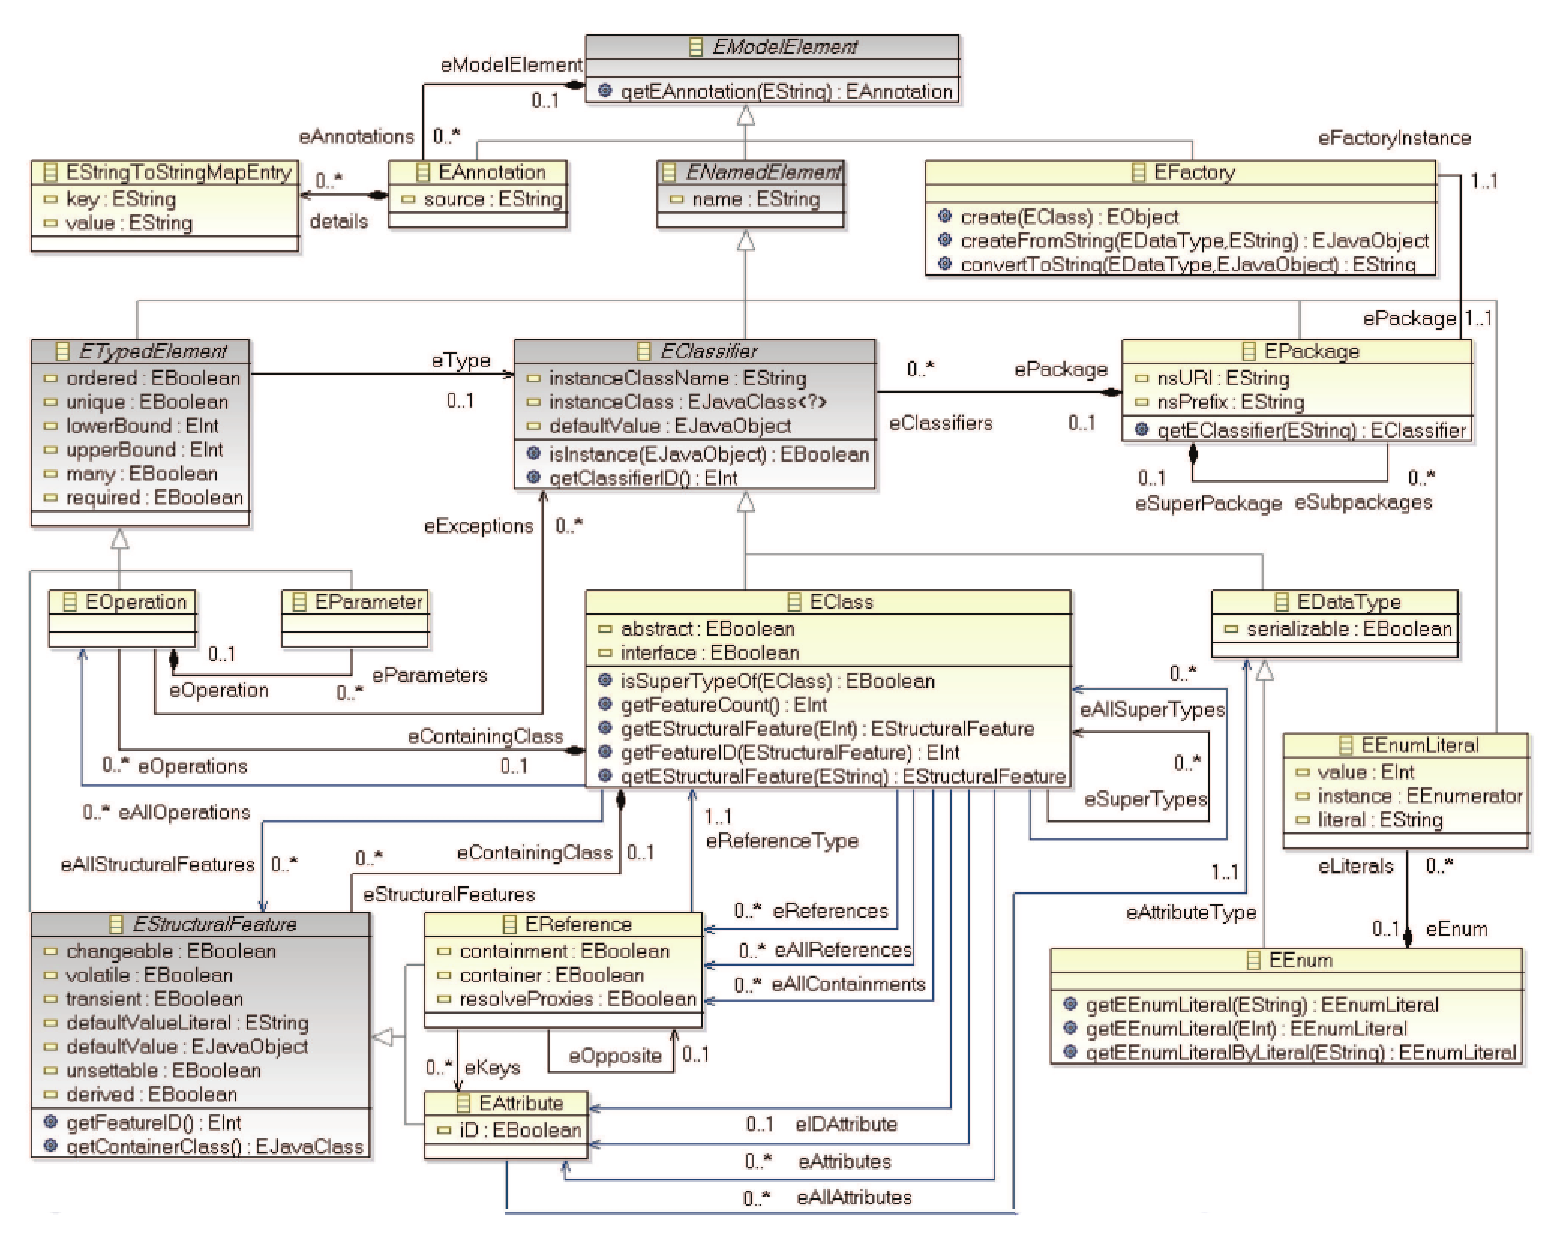
\includegraphics [width=135mm, height=120mm]{imagenes/ecore.eps}
\end{center}
\caption{Especificación del formato Ecore.}
\label{fig:ECORE}
\end{figure} 


\section{La Transformación}
\label{La Transformacion}

... hablar de la definiciones de las relaciones. Mostrar las partes de codigo mas relevantes de las relaciones.

